%%%%%%%%%%%%%%%%%%%%%%%%%%%%%%%%%%%%%%%%%%%%%%%%%%%%%%%%%%%%%%%%%%
%%%%%%%% ICML 2017 EXAMPLE LATEX SUBMISSION FILE %%%%%%%%%%%%%%%%%
%%%%%%%%%%%%%%%%%%%%%%%%%%%%%%%%%%%%%%%%%%%%%%%%%%%%%%%%%%%%%%%%%%

% Use the following line _only_ if you're still using LaTeX 2.09.
%\documentstyle[icml2018,epsf,natbib]{article}
% If you rely on Latex2e packages, like most moden people use this:
\documentclass{article}

% For figures
\usepackage{graphicx} % more modern
%\usepackage{epsfig} % less modern
\usepackage{subfigure} 
\usepackage{natbib}
\usepackage{amssymb}
\usepackage{amsmath}
\usepackage{amsfonts}
\usepackage{amsthm}
\usepackage{mathtools}
\usepackage{lipsum}% http://ctan.org/pkg/lipsum
\usepackage{multicol}% http://ctan.org/pkg/multicols
\usepackage{graphicx}% http://ctan.org/pkg/graphicx
%\usepackage{algorithm2e}
% For algorithms
\usepackage{algorithm}
\usepackage{algorithmic}

% As of 2011, we use the hyperref package to produce hyperlinks in the
% resulting PDF.  If this breaks your system, please commend out the
% following usepackage line and replace \usepackage{icml2013} with
% \usepackage[nohyperref]{icml2013} above.
\usepackage{hyperref}

% Packages hyperref and algorithmic misbehave sometimes.  We can fix
% this with the following command.
\newcommand{\theHalgorithm}{\arabic{algorithm}}

% Employ the following version of the ``usepackage'' statement for
% submitting the draft version of the paper for review.  This will set
% the note in the first column to ``Under review.  Do not distribute.''

\usepackage{icml2013} 
% Employ this version of the ``usepackage'' statement after the paper has
% been accepted, when creating the final version.  This will set the
% note in the first column to ``Proceedings of the...''
% \usepackage[accepted]{icml2013}
\newtheorem{theorem}{Theorem}
\newtheorem{lemma}{Lemma}
\newtheorem{remark}{Remark}
\newtheorem{corollary}{Corollary}

% The \icmltitle you define below is probably too long as a header.
% Therefore, a short form for the running title is supplied here:
\icmltitlerunning{2-bits Compressive Sensing with Use Case in Radio Astronomy}

\begin{document} 
\setlength{\abovedisplayskip}{5.5pt}
\setlength{\belowdisplayskip}{6pt}

\twocolumn[
\icmltitle{2-bits Compressive Sensing with Use Case in Radio Astronomy}

% It is OKAY to include author information, even for blind
% submissions: the style file will automatically remove it for you
% unless you've provided the [accepted] option to the icml2013
% package.
\icmlauthor{Nezihe Merve G\"{u}rel}{nezihe.guerel@inf.ethz.ch}
\icmladdress{Eidgen�ssische Technische Hochschule Z�rich,
            314159 Pi St., Palo Alto, CA 94306 USA}
\icmlauthor{Your CoAuthor's Name}{email@coauthordomain.edu}
\icmladdress{Their Fantastic Institute,
            27182 Exp St., Toronto, ON M6H 2T1 CANADA}

% You may provide any keywords that you 
% find helpful for describing your paper; these are used to populate 
% the "keywords" metadata in the PDF but will not be shown in the document
\icmlkeywords{compressed sensing, low precision, iterative hard thresholding, radio astronomy, fpga}

\vskip 0.3in
]

\begin{abstract} 
Iterative Hard Thresholding (IHT) algorithm offers near optimal recovery of compressible signals sampled below the Nyquist rate. IHT, however, seems to have a computational bottleneck when applied to the compressed sensing recovery problems with general (non-Gaussian) dense measurement matrices. To relieve this, we propose to compress the measurement matrix by quantizing the bit-widths of its entries at each iteration. This low precision framework results in runtime efficiency on hardware yet still maintaining the stability and performance guarantees of the algorithm. To demonstrate this, we first derive theoretical error bounds for sparse signal recovery. Under certain constraints, low precision IHT is shown to converge with performance guarantees. We then illustrate through empirical experiments the potential for radio interferometry imaging with achievement of 7.7x speed up on Field-Programmable Gate Array. An application to LOFAR, the low frequency array in Netherlands, leads to a better resolution of the sky sources recovered with order of magnitude speed up. 
\end{abstract} 
\section{Introduction}
The Square Kilometre Array (SKA) will form, when fully deployed, the largest, the most sensitive and the fastest radio telescope ever built with thousands of dishes and over a square kilometres of collecting area. The most powerful radio telescope on Earth that has ever known, the SKA combines thousands of antennas at various locations spread over an extensive area on the ground. The data collected by the antennas is immense to be efficiently processed further in the operational chain. The estimated raw data throughput by mid 2020s is 62 exabytes: 20 times higher than the global email traffic. The SKA thus demands advanced functional and operational capabilities such as engineering, algorithms, instrument calibration, storage and many others~\cite{hu, rik2016ska}. 

This work proposes to reduce the precision of floating-point data representations by reducing the bit widths, hence enabling more information transfer and processed at the Central Signal Processor of telescope. We first linearize image acquisition process by formulating the problem in compressive sensing framework, and under certain constraints, derive near-optimal guarantees for precise sky recovery. Our approach is a general framework and can facilitate further sparse reconstruction problems demanding high processing capability in practice. We demonstrate the power of our proposal on LOFAR, where we achieve significant practical speedup.
%radio interferometry encounters the task of inferring from measured information


\subsection{Compressive Sensing}
The rapidly emerging field of compressive sensing (CS)~\cite{donoho2006cs, candes2006cs, candes2006cs2} is a foundational technique in sparse signal reconstruction. CS offers a range of efficient algorithms acquiring high dimensional signals from inaccurate and incomplete samples when the structure is known a priori: sparsity. Many real-life problems of medical imaging, interferometry, video, spectroscopy and genomic data analysis  benefit these techniques, i.e., they are practically well-approximated by sparse signals.

% 1- CS
In mathematical terms, the standard CS problem is formulated as follows. Let a sparse or approximately sparse signal ${\bf x}\in \mathbb{R}^N$ be sampled with a linear sampling operator ${\bf \Phi}^{M\times N}$. In matrix notation, the vector of measurements ${\bf y} \in \mathbb{C}^M$ is
\begin{equation}\label{CS_model}
 {\bf y} =  {\bf \Phi}  {\bf x} + {\bf e}
\end{equation}
where ${\bf e}$ is the observation noise and $M < N$.

The CS algorithms iteratively build up a sparse estimate ${\bf x}$ such that ${\bf \Phi}  {\bf x}$ well approximates ${\bf y}$, that is,  $\| {\bf y}- {\bf \Phi}  {\bf x} \|_2$ is small. The sparsity constraint imposed on ${\bf x}$ radically overcomes this ill-posed problem yet computationally NP-hard due to its combinatorial nature. Hence CS is often synonymous to convex relaxation of $\ell_0$-based optimization, or a collection of thresholding and greedy methods such as Iterative Hard Thresholding (IHT) \cite{blumensath2008iht, blumensath2009iht} and Compressive Sampling Matching Pursuit (CoSaMP) \cite{needel2008cosamp}. The past decade has seen an explosion of discoveries on CoSaMP and IHT and avalanche of results obtained by~\cite{liu2017dualiht, yuan2014ht, yuan2016htp, blumensath2013cs, needel2008cosamp} and the references therein. There, a comprehensive analysis is performed to derive the provable performance guarantees of such sparsity-constrained minimization methods, namely, the convergence to fixed points of $\ell_0$-regularized cost functions and the optimality of such approximation. They however face several challenges when applied to real-life problems: for provable guarantees (1) the measurement matrix ${\bf \Phi}$ is required to satisfy the Restricted Isometry Property (RIP)~\cite{candes2008rip, chartrand2008rip} when operating onto sparse vectors, (2) the sparsity level has to be chosen appropriately. A simple yet effective strategy is suggested by \cite{blumensath2010niht} that massively relieves the limitations listed above: a step size parameter is introduced to the traditional IHT~\cite{blumensath2008iht}. This simple refinement alleviates the RIP condition imposed on ${\bf \Phi}$ hence enabling rigorous guarantees for a broader class of problems in practice. 
\subsection{Technical contributions}
 We consider the sparse signal recovery problem in~\ref{CS_model} described as: for given ${\bf y}$ and ${\bf \Phi}$, find coefficients ${\bf x}$ minimizing the cost function
 \begin{equation}\label{cost_function}
     \|{\bf y} - {\bf \Phi x} \|_2^2 \ \ \rm{subject \ to \ \|{\bf x} \|_0 \leq s}
 \end{equation}
 where $\|{\bf x} \|_0 = |\rm{supp}({\bf x})| = |\{i: x_i\neq 0 \}|$.
 
 Under certain constraints, normalized IHT is guaranteed to approximate ${\bf x}$ with high accuracy. We rather consider the properties of this algorithm in a lossy compression scheme: the data ${\bf y}$ and ${\bf \Phi}$ consisting of floating point values undergoes a stochastic rounding process to a small set of integer levels denoted by $Q$. That is, we recover ${\bf x}$ using a modified update rule of normalized IHT:
 \begin{equation}
     {\bf x}^{[n+1]} = H_s({\bf x}^{[n]} + \mu^{[n]}Q({\bf \Phi})(Q({\bf y}) - Q({\bf \Phi}){\bf x}))
 \end{equation}
where $H_s({\bf x}): \mathbb{C}^n \rightarrow \mathbb{C}^n$ the nonlinear operator that preserves the largest $s$ (in magnitude) entries of {\bf x} and sets the remaining to zero. 
 
 The core contribution of this work is two fold in theory and algorithm as highlighted in below: 
 
     $\bullet$ Low precision IHT: we established a rigorous analysis on the quality of recovery by bounding the approximation error. To our knowledge, compression performed on the measurement matrix has not been reported elsewhere in liteature.\\
     $\bullet$ We formulate radio interferometry imaging as a CS problem and employed low precision IHT on a real telescope. Our experiments demonstrated that sky map can still be recovered with no or small accuracy lost by using only 2-bits to represent the data points with 7.7x speed-up on FPGA.
     
{\bf Organization. }
The rest of this paper is organized as follows. In Section \ref{section_related_work} we briefly review some relevant work. Section \ref{section_iht} serves an introduction to IHT, including the theoretical performance guarantees. Section~\ref{section_lpiht} describes how the low precision framework is applied to IHT and presents derivable theoretical guarantees for such a lossy scheme, and devises our approach for real telescopes. Section~\ref{section_experiments} reports the numerical evaluation results. Section~\ref{section_discussion} concludes the overview. All the technical proofs are deferred to the supplementary material.

\section{Related work}\label{section_related_work}
The current studies predominantly revolve around "low precision Stochastic Gradient Descent (SGD)" covering a spectrum of machine learning tasks and models. Quantizing gradients, Buckwild!~\cite{desa2015hogwild} established convergence guarantees of low precision SGD achieving significant speed-up on CPU when solving convex problems. \cite{alistarh2016qsgd}, which mainly focuses on the trade-off between communication and convergence, refines this to quantized non-convex cases. A follow-up, \cite{zhang2017zipml} further extends this framework to an {end-to-end} quantization scheme that governs all data components. \cite{seide2014sgd1bit, hubara2016qsnn, rastegari2016binarycnn,zhou2016cnn, miyashita2016cnn, li2016twn, gupta2015dl} mainly concern of generalization of {\it end-to-end} quantization to training deep learning models. 

Recently, however, there emerge a wave of studies that has successive attempts applying the low precision framework to compressive sensing problems.~\cite{boufounos20091bitcs} demonstrate the sparse signals can be recovered with a scale factor when measurements preserve only sign information.~\cite{ai20121bitcs, davenport20121bit} exhibit that approximately sparse signals can be robustly recovered from single-bit measurements sampled with a sub-gaussian distribution.~\cite{jacques20111bit, laska20111bitcs} study the similar setting with a Gaussian measurement matrix the so called Binary IHT. \cite{plan20111bitcs, plan20121bitcs} propose a computationally tractable and optimal recovery of 1-bit compressive sensing problem. \cite{recht20121bitcs, gopi20131bitcs} present provable theoretical guarantees to identify support recovery of high dimensional sparse signals for 1-bit measurements. 

Multi-level quantization of measurement for CS problems, therefore, exhibit a great empirical success. The analysis of such heuristics is yet challenging. In this paper, a successive application of low precision framework to CS, particularly IHT, is shown to possess rigorous theoretical guaratees, potentially allowing more efficient information processing in large scale applications. To distinct from the prior proposals listed above, we achieve this by quantizing not only measurements but also measurement matrix.

Another line of research on concerns accelerating the sparse recovery algorithms \cite{blumensath2011aiht, wei2015fiht, blanchard2013iht, cevher2011ht, liu2017dualiht}. need to bridge to hardware here












\section{Preliminaries}\label{section_iht}
In this section, we review the preliminary results on the normalized IHT algorithm introduced by~\cite{blumensath2010niht, blumensath2012greedy}.

{\it Notation:} Scalars are denoted by italics, vectors by bold lower-case and matrices by bold upper-case. For all ${\bf x}= (x_1, \hdot, x_n) \in \mathbb{R}^n$, we denote by $\|{\bf x}\|_p$ the standard operator norm. Finally, let ${\bf \Phi}_{m, n}\in \mathbb{C}^{M\times N}$ denote its element in $m$'th row and $n$'th column.
\subsection{Iterative Hard Thresholding} 
Let ${\bf x}^{[0]} = 0$, the normalized IHT has the following update rule per iteration
\begin{equation}\label{iht_update_rule}
{\bf x}^{[n+1]} = H_s({\bf x}^{[n]} + \mu^{[n]}{\bf \Phi}({\bf y}-{\bf \Phi}{\bf x}^{[n]})),
\end{equation}
where $\mu^{[n]}>0$ is the adaptive step size parameter. %Under certain conditions, the normalized IHT converges to a local minimum of the optimization problem
%\begin{equation}\label{cost_function}
%    \textrm{min} \|{\bf y}-{\bf \Phi x} \|_2^2
%\ \ \ {\textrm{subject \ to }}\ \ \|{\bf x}\|_0 \leq s.
%\end{equation}

\subsection{Convergence} 
The analysis of hard thresholding algorithms heavily relies on the scaling properties of ${\bf \Phi}$. More precisely, the convergence to a local minimum of the cost function \ref{cost_function} as well as the quality of such approximation were proven under certain conditions on ${\bf \Phi}$. To be more concrete on these conditions, one must often deal with non-symmetric Restricted Isometry Property (RIP), namely, a matrix ${\bf \Phi}$ satisfies non-symmetric RIP if
\begin{equation}\label{rip}
\alpha_{s} \leq \frac{\|{\bf \Phi} {\bf x}\|_2}{\|{\bf x}\|_2} \leq \beta_{s}
\end{equation}
for all ${\bf x}: \|{\bf x}\|_0 \leq s$, and some $\alpha_s, \beta_s \in \mathbb{R}$ such that $0<\alpha_s\leq \beta_s$. the so-called Restricted Isometric Constants (RICs).
\begin{remark}\label{remark_noise_amp}
The convergence of normalized IHT depends conditionally on the step size parameter $\mu^{[n]}$ unlike the traditional IHT approach where $\mu^{[n]}=1$.
While the traditional approach requires a re-scaling of measurement matrix such that $\|{\bf \Phi}\|_2 <1$ to ensure convergence, introducing a step size parameter enables the arbitrary scaling of ${\bf \Phi}$ hence relaxing the bounds of its norm. The role of $\mu^{[n]}$ here is to compensate for this re-scaling by accordingly avoiding undesirable amplification of noise, i.e., the ratio of $\|{\bf \Phi x}\|_2/\|{\bf e}\|_2$ remains unchanged. 
\end{remark}
The main convergence result can be stated as follows.
\begin{theorem}\label{theorem_convergence_IHT}
{\rm{\cite{blumensath2012greedy}}}\\ 
Let ${\bf \Phi}$ is of full rank and $s\leq m$. If $\beta_{2s}\leq\mu^{-1}$, then normalized IHT converges to a local minimum of \ref{cost_function}.
\end{theorem}
\subsection{Step Size Determination} 
While setting the step size parameter, the condition that $\beta_{2s}\leq\mu^{-1}$ ensuring convergence poses the following challenge. To date, there is no universal strategy known to check if the RIP holds for an arbitrary measurement matrix in a computationally efficient manner. Similar discussion holds for attaining the RICs, i.e., ${\beta_s}$ and $\alpha_s$, associated with the measurement matrix ${\bf \Phi}$. It could however be shown that, under certain conditions, randomly constructed measurement matrices can satisfy
the RIP with high probability~\cite{candes2008rip, chartrand2008rip}. Still, it remains a bottleneck for a more general class of
measurement matrices. Without losing the main track, here we intend to review a more generic strategy for step size determination.

If the support is fixed, a natural strategy to set the step size adaptively is~\cite{blumensath2010niht}
\begin{equation}\label{step_size}
   \mu^{[n]} = \frac{{\bf g}^T_{\Gamma^{[n]}}{\bf g}_{\Gamma^{[n]}}}{{\bf g}^T_{\Gamma^{[n]}}{\bf \Phi}^T_{\Gamma^{[n]}}{\bf \Phi}_{\Gamma^{[n]}}{\bf g}_{\Gamma^{[n]}}}
\end{equation}
where ${\bf g}^{[n]} = {\bf \Phi}^T({\bf y}-{\bf \Phi x}^{[n]})$. Clearly, the maximal reduction in cost function can then be attained. However, if the support of ${\bf x}^{[n+1]}$ differs than that of ${\bf x}^{[n]}$, the sufficient condition to guarantee convergence 
\begin{equation}
    \mu^{[n]} \leq(1-c) \frac{\|{\bf x}^{[n+1]}-{\bf x}^{[n]} \|_2^2}{\|{\bf \Phi}({\bf x}^{[n+1]}-{\bf x}^{[n]}) \|_2^2},
\end{equation}
for any small constant $c$.

If the above condition is not met, a new proposal for ${\bf x}^{[n+1]}$ can be calculated by using $\mu^{[n]}\leftarrow{\mu^{[n]}/(k(1-c))}$, where $k$ is a shrinkage parameter such that $k>1/(1-c)$.
% In a series of papers [...], extensive research effors have been made and strong theoretical guarantees were derived. Here we state the most refined recovery error bounds.
This adaptive setting of step size parameter is shown to provide RIP-invariant convergence result as follows.
\begin{theorem}\label{guarantee_niht}
{\rm{\cite{blumensath2010niht}}}\\
Consider a noisy observation ${\bf y} = {\bf \Phi x} + {\bf e}$ with an arbitrary vector {\bf x}. If rank({${\bf \Phi}$}) = m and rank(${\bf \Phi}$_{\Gamma}) = s \ $\forall \Gamma:\ |\Gamma| = s$, then the normalized IHT algorithm converges to a local minimum of the cost function~\ref{cost_function}. Also, assume ${\bf \Phi}}$ is non-symmetric RIP$_{2s}$ and let $\gamma_{2s} = \beta_{2s}/\alpha_{2s}-1$. If $\gamma_{2s} \leq {1}/{8}$, then
\begin{equation}
    \| {\bf x}-{\bf x}^n\|_2 \leq 2^{-n}\| {\bf x}^s\|_2 + 8 {{\bf \epsilon}_s}\label{niht_error_bound}
\end{equation} where \begin{equation}
     {{\bf \epsilon}_s} =  \| {\bf x}-{\bf x}^s\|_2 + \frac{\| {\bf x}-{\bf x}^s\|_1}{\sqrt{s}}+\frac{1}{\beta_{2s}}\|{\bf e} \|_2.
\end{equation}
After at most $n^*=\log_2(\|{\bf x}^s\|_2/ {\bf \epsilon}_s)$ iterations, the recovery error bound in \ref{niht_error_bound} can be further simplified to
\begin{equation}
   \| {\bf x}-{\bf x}^n\|_2 \leq 9 {{\bf \epsilon}_s}.
\end{equation}
\end{theorem}
The above result suggests that, after a sufficiently large number of executions, the reconstruction error is induced only by the noise ${\bf e}$ and that ${\bf x}$ is not exactly s-sparse.
\section{Low Precision Iterative Thresholding}\label{section_lpiht}
In this section, we present the proposed approach and establish rigorous guarantee for signal recovery performance. The key development here is that, by reducing the bit widths of the data points, we still obtain near-optimal recoveries. 

As introduced earlier, let ${\bf x}^{[0]} = 0$ and use iteration
\begin{equation} \label{modified_update_rule}
  {\bf x}^{[n+1]} = H_s\big({\bf x}^{[n]}+\hat{\mu}^{[n]} Q_b(\boldsymbol{\Phi})(Q_b({\bf y})-Q_b(\boldsymbol{\Phi}){\bf x}^{[n]})\big)  
\end{equation}
where $Q(\cdot)$ is the quantization function that maps single-precision floating-points onto a codomain where each element has $b$-bits precision.

{\bf Quantization Scheme:} We employ a stochastic quantization function denoted with $Q_b({\bf v})$, where ${\bf v}=(v_1, v_2, .., v_d) \in \mathbb{R}^d$ is an arbitrary vector and $b$ is the total number of bits used to represent it. {\bf v} can then be quantized into $l=2^b$ levels as follows. Let $\ell_i$, $i\in \{1, 2, ..., l-1 \}$ denote $l$ equally spaced points on $[-1, 1]$ such that $\ell_1= -1$, $\ell_l= +1$ and $\ell_1\leq\ell_2 \leq ... \leq \ell_l$, also $v_j$ for $j\in \{1, 2, ..., d \}$ fall into the interval $[\ell_i, \ell_{i+1}]$. Then we assign the probabilities to the nearest levels as
\[
    Q_b(v_j) = \left\{\begin{array}{lr}
        \ell_i, & \textrm{with probability} \ \frac{\ell_{i+1}-v_j}{\ell_{i+1}-\ell_i}\\
        \ell_{i+1},&\textrm{otherwise}.  \ \ \ \  \ \ \ \ \ \ \ \ \ \ \ \ \ \ 
        \end{array}
\]
  
Remark that the above equation yields that the quantization operation $Q(\cdot)$ is unbiased, i.e., $\mathbb{E}[Q_b({\bf v})] = {\bf v}$. Also, let $\hat{{\bf v}}$ represent the quantized ${\bf v}$ and drop $Q_b(\cdot)$ to simplify notational burden. The detailed steps of the algorithm is then given in Algorithm \ref{low_precision_iht}.
\begin{algorithm}[h!]
   \caption{Low Precision Iterative Thresholding}
   \label{low_precision_iht}
\begin{algorithmic}
   \STATE {\bfseries Input:} The set of low precision measurement matrices $\{ \hat{\bf \Phi}_1, \hat{\bf \Phi}_2, ...\hat{\bf \Phi}_{2n^*}\}$, measurements $\hat{\bf y}$, sparsity parameter $s$, number of iterations $n^*$ 
   \REPEAT
   \STATE Initialize ${\bf x} = 0$, $\Gamma^{[1]} = \rm{supp}\big (H_s(\hat{\bf \Phi}_1^{\dagger}{\hat{\bf y}})\big)$.
   \FOR{$n=1$ {\bfseries to} $n^*$}
   \STATE ${\bf g}^{[n]} = {\hat{\bf \Phi}}_{2n-1} \big(\hat{{\bf y}}-{\hat{\bf \Phi}}_{2n}{\bf x}^{[n]}\big)$
   \STATE $\hat{\bf \mu}^{[n]} = ({\bf g}^{\dagger}_{\Gamma^{[n]}}{\bf g}_{\Gamma^{[n]}})/({\bf g}^{\dagger}_{\Gamma^{[n]}}{\bf \Phi}^{\dagger}_{\Gamma^{[n]}}{\bf \Phi}_{\Gamma^{[n]}}{\bf g}_{\Gamma^{[i]}})$
   \STATE ${\bf x}^{[n+1]} = H_s({\bf x}^{[n]} + \hat{\bf \mu}^{[n]} {\bf g}^{[n]})$
   \STATE $\Gamma^{[n+1]} = \rm{supp}({\bf x}^{[n+1]})$
   \STATE tbc
   \ENDFOR
   \UNTIL $n = n^*$
\end{algorithmic}
\end{algorithm}

{\bf Convergence:} The modified algorithm attains a local minimum of the cost function $\mathbb{E} [ \| \hat{\bf y} - \hat{\bf \Phi}{\bf x}\|_2^2]$ such that $\|{\bf x}\|_0 \leq s$. This can be majorized by the following surrogate objective function 
\begin{equation*}
    \begin{split}
        \mathbb{E} [\|\mu^{0.5}\hat{\bf y} -   \hat{\bf \Phi}{\bf x}\|_2^2+ \|{\bf x} 
    - {\bf x}^{[n]} \|_2^2
    - \|\mu^{0.5}\hat{\bf \Phi}({\bf x}- {\bf x}^{[n]}) \|_2^2] 
    \end{split}
\end{equation*}
whenever $\| \mu^{0.5}\hat{\bf \Phi}\|_2^2 <1$. If this condition is met, the minimizer of the above surrogate objective: ${\bf x}^{[n+1]}$ ensures that $\mathbb{E} [\| \hat{\bf y} - \hat{\bf \Phi}{\bf x}^{[n+1]}\|_2^2] \leq \mathbb{E}[ \| \hat{\bf y} - \hat{\bf \Phi}{\bf x}^{[n]}\|_2^2]$. Moreover, by using the arguments of~\cite{blumensath2008iht}, \ref{modified_update_rule} can be shown to minimize the expected cost $\mathbb{E} [ \| \hat{\bf y} - \hat{\bf \Phi}{\bf x}\|_2^2]$. For deterministic quantization scheme, Theorem~\ref{theorem_convergence_IHT} ensures the convergence to a fixed point.

{\bf Computational Complexity:} The iterative thresholding algorithm involves two vector additions and two dense matrix multiplication as well as a thresholding operation per iteration, and this is doubled due to step size search. Low precision approach however reduces memory requirements significantly. (we need to improve here)
 
{\bf Conditions on ${\Phi}$:} The restricted isometry property holds for the quantized measurement if
\begin{equation}
    \hat{\alpha}_{s} \leq \frac{\|\hat{{\bf \Phi}} {\bf x}\|_2}{\|{\bf x}\|_2} \leq \hat{\beta}_{s}
\end{equation}
$\forall {\bf x}: \| {\bf x}\|_0 \leq s$. Furthermore, the RICs: $\hat{\alpha}_s$ and $\hat{\beta}_s$ can be re-scaled accordingly with $\hat{\bf \Phi}$.

%{\bf Bounds of $\$:} 
%The step size $\hat{\mu}^{[n]}$ is required to counteract the scaling of $\hat{{\bf \Phi}}$ such that $\|\hat{\mu}^{0.5} \hat{\bf\Phi}\|_2^2 <1$ to ensure the convergence. 
%This adaptive step size setting yields the trivial bound on $\mu$ as~\cite{blumensath2012greedy}
%\begin{equation}
 %  1/\hat{\beta}_{2s}^2\leq  1/\hat{\beta}_s^2 < \hat{\mu}^{[n]} < 1/\hat{\alpha}_s^2 \leq 1/\hat{\alpha}_{2s}^2.
%\end{equation}
%Moreover, using \ref{step_size} in the low precision setting, we can initially determine $\hat{\mu}^{[n]}$ to guarantee the convergence without requiring the knowledge of the restricted isometry constants.
\subsection{Performance Guarantees}
Convergence is necessary to guarantee the existence of a stable scheme. However, the recovery performance of such algorithms is of our primary interest. The following theorem states the recovery error by explicitly exhibiting the component introduced by the quantization.
\begin{theorem}\label{main_theorem_TH}
Given a noisy observation ${\bf y} = {\bf \Phi x}+{\bf e} $ where ${\bf x}$ is an arbitrary vector with $\|{\bf x} \|_0 \leq s$ and let $H_s({\bf x}) = {\bf x}^s$ with $s\leq m$. Let $\hat{\bf \Phi}$ satisfies the nonsymmetric RIP with $\hat{\alpha}_s$ and $\hat{\beta}_s$ where $\hat{\gamma}_{2s} = \hat{\beta}_{2s}/\hat{\alpha}_{2s} -1 \leq 1/16$. If the normalized IHT algorithm is used at low precision we have
\begin{equation}\label{main_theorem}
\begin{split}
        \mathbb{E}[\|\hat{{\bf x}}^{[n+1]}-{\bf x}^s\|_2]  
        \leq &2^{-n}\|{\bf x}^{s}\|_2  + 10 {\epsilon}_s + 5 {\epsilon}_q
\end{split}
\end{equation}
with 
\begin{equation}
 {\epsilon}_s = \frac{1}{\beta_{2s}}\|{\bf e} \|_2 +\bigg  [ \|{\bf x}-{\bf x}^s \|_2 + \frac{\|{\bf x}-{\bf x}^s \|_1}{\sqrt{s}}\bigg]    
\end{equation}
and
\begin{equation}
 {\epsilon}_q = \frac{\sqrt{m}}{\hat{\beta}_{2s}}\Big ( \frac{\| {\bf x}^s\|_2}{2^{b_{\bf \Phi}-1}}+\frac{1}{2^{b_{\bf y}-1}} \Big )
\end{equation}
where $b_{\bf \Phi}$ and $b_{\bf y}$ are the numbers of bits to represent ${\bf \Phi}$ and ${\bf y}$, respectively.
\end{theorem}

A natural stopping criterion is $n^* = \lceil \log_2 (\|{\bf x}^s \|_2/\epsilon_s)\rceil$ where the algorithm compute a successive approximation to ${\bf x}^s$ with accuracy
\begin{equation}
    \mathbb{E}[\|{\bf x}^{[n^*]}-{\bf x}^s \|_2] \leq 11\epsilon_s + 5\epsilon_q.
\end{equation}
The error bound above is actually oversimplified, our proof in the supplementary material is slightly more delicate. Namely, the quantization operator introduces only $\frac{5}{\beta
{2s}} \|{\bf e} \|_2$ into $8 {\epsilon}_s$ in \ref{niht_error_bound}, which is tighter than $10 {\epsilon}_s$ in~\ref{main_theorem}.

We now examine the error bound presented in Theorem~\ref{main_theorem_TH}. The low precision IHT will asymptotically provide a sparse approximation of ${\bf x}$ up to the multiples of $ {\epsilon}_s$ and $ {\epsilon}_q$ involving the noise term ${\bf e}$, the approximation error on how well ${\bf x}$ can be represented by a sparse vector ${\bf x}^s$ and the corruption introduced by the quantization operator. This makes intuitive sense yet still requires the understanding of our limits on the accuracy of results achievable at low precision. Here we highlight the main limitations.

{\bf Condition on $\hat{\boldsymbol{\gamma}}_{2s}$:} In comparison to the unmodified algorithm, the condition under which the performance guarantee holds is stricter in our approach, i.e., $\hat{\gamma}_{2s}\leq 1/16$ where it was ${\gamma}_{2s}\leq 1/8$ in Theorem \ref{guarantee_niht}. In practice, this can be altered with a suitable transformation of $\hat{\bf \Phi}$ such that $\hat{\gamma}_{2s}\leq 1/16$ is satisfied. Alternatively, a closer look into the derivation in the supplementary material reveals that there exists finite constants $c_1$ and $c_2$ such that $\mathbb{E}[\|{\bf x}^{n^*}-{\bf x}^s \|_2] \leq c_1\epsilon_s + c_2\epsilon_q$ when $\hat{\gamma}_{2s}\leq 1/8$. For a wide class of problems, an accurate approximation to ${\bf x}^s$ can still be recovered after sufficient number of iterations.
%One might argue that it can potentially amplify noise yet from changing $\gamma_{2s}$ from $1/8$ to $1/16$ 

%We also monitor $\hat{\gamma}_{2s}$ by using the strategy described in ref.

%can easily be verified in a computationally efficient manner
{\bf Natural limitations on $\hat{\boldsymbol{\beta}}_{2s}$:} In both low and high precision settings, the measurement matrix ${\bf \Phi}$ is scale-invariant and rigorous theoretical guarantee is achievable provided its scaling onto sparse vectors is confined in certain intervals, i.e., $\hat{\gamma}_{2s}\in [0, 1/16]$. As introduced in Remark \ref{remark_noise_amp}, even this condition is met, there still remains a further limitation by the noise: ${\bf e}$. That is, the signal-to-noise ratio of $\|\hat{\bf \Phi} {\bf x} \|_2/\|{\bf e} \|_2$ will be amplified upon a down-scaling of $\hat{\bf \Phi}$. Re-scaling ${\bf y}$ can accordingly overcome this up to some level. (not sure it it's clear)

{\bf Further limitation on $\hat{\boldsymbol{\beta}}_{2s}$ due to quantization:} The recovery error bound satisfying \ref{main_theorem} depends on the error term of high precision IHT: $ {\epsilon_s}$ and the quantization error: $ {\epsilon}_q$ that is inversely proportional to $\hat{\beta}_{2s}$. For sufficiently large $\hat{\beta}_{2s}$ that compensates for $\sqrt{M} \|{\bf x}^s \|_2$, the low precision approach appears competitive with the unmodified algorithm where the recovery error is bounded by $9\epsilon_s$ in~\ref{niht_error_bound}. Furthermore, the scaling-invariant property of the measurement matrix $\hat{\bf \Phi}$ permits us to scale up $\hat{\beta}_{2s}$ by still retaining the strong recovery result similar to that of high precision algorithm. An arbitrary scaling of $\hat{\bf \Phi}$ has no effect on the condition $\hat{\gamma}_{2s}\leq 1/16$. We however have strong theoretical guarantee for the recovery holds if the low precision algorithm operates in a regime where both the condition of $\hat{\gamma}_{2s}\leq 1/16$ holds and ${\epsilon}_q$ is relatively small.

From quantization point of view, re-scaling of the ${\bf y}$ and $\hat{\bf \Phi}$ has no necessity,
otherwise the constant factor weighting ${\epsilon}_q$ will change. A small factor naturally reduces the quantization error yet imposes some mild conditions on $\hat{\beta}_{2s}$. Namely, $\hat{\beta}_{2s}$ can not arbitrarily, instead is required to satisfy that all entries of ${\bf y}$ and $\hat{\bf \Phi}$ are contained in $[-1, 1]$.

% \subsection{An Alternative Approach}
% The normalized IHT offers an adaptive step size tuning to ensure maximal reduction in the cost function at each iteration, yet doubling the computational cost. We instead propose using a constant step size that guarantees the convergence, that is, $\hat{\mu}=\frac{k}{\|{\bf \Phi} \|_{\mathcal{F}}}$ with $0<k<1$. This modification might increase the convergence time but counteracts the additional cost introduced by iterative tuning of ${\mu}^{[n]}$. We therefore have the following version.
% \begin{theorem}
% Let ${\bf \Phi}$ satisfies the non-symmetric RIP with RICS $\alpha_s$ and $\beta_s$. If normalized IHT uses a constant step size $\mu = 1/(8\beta_{2s})$ then
% \begin{equation}\label{secondary_theorem}
% \begin{split}
%         \mathbb{E}[\|\hat{{\bf x}}^{[n+1]}-{\bf x}^s\|_2]  
%         \leq &2^{-n}\|{\bf x}^{s}\|_2  + 10 {\epsilon}_s + 5 {\epsilon}_q
% \end{split}
% \end{equation}
% with 
% \begin{equation}
%  {\epsilon}_s = \frac{1}{\beta_{2s}}\|{\bf e} \|_2 +\bigg  [ \|{\bf x}-{\bf x}^s \|_2 + \frac{\|{\bf x}-{\bf x}^s \|_1}{\sqrt{s}}\bigg]    
% \end{equation}
% and
% \begin{equation}
%  {\epsilon}_q = \frac{\sqrt{m}}{\hat{\beta}_{2s}}\Big ( \frac{\| {\bf x}^s\|_2}{2^{b_{\bf \Phi}-1}}+\frac{1}{2^{b_{\bf y}-1}} \Big )
% \end{equation}
% \end{theorem}

{\bf Comparison to other state-of-art methods:} Compressive sensing literature covers a range algorithms such as $\ell_1$-minimization, greedy and thresholding-based methods that have certain properties weighted against each other. In~\cite{blumensath2010niht}, CoSaMP, normalized IHT and $\ell_1$-minimization exhibit similar empirical performance when applied to the problems with dense Gaussian matrices. Moreover, after a simple modification of step size parameter, IHT has became compatible with these powerful methods with similar provable guarantees~\cite{blumensath2012greedy}. 

We test empirical performance of low precision IHT on a simple toy examples using a Gaussian measurement matrices and refer to the supplementary material for further discussion. 
















\subsection{Application to Radio Astronomy}
Radio interferometers at various locations on the ground record radio waves emitted by the celestial sources over a certain time interval, then store and process it all in order to deduce a sky image. Interferometers first estimate the cross-correlation between the time series measurements that is called visibilities, and sky image is estimated by the so-called {CLEAN} algorithm~\cite{hogbom1974clean}. {CLEAN} is a greedy pursuit technique, deconvoluting the inverse Fourier transform of visibilities and forming a sky map by iteratively removing a fraction of the highest peak convolved with an instrument based point spread function. {\it CLEAN} is a simple and easy-to-implement imaging technique, yet radio interferometers are formed as a CS problem, for example, by~\cite{wiaux2009csforra, wenger2010csforra, li2011deconvolution} inspired by its recovery success in noisy environments.

Let sky be observed by employing $L$ antennas over a stationary time interval (STI) where the earth rotation is negligible. Also, we denote the vectorized sky image by ${\bf x} \in \mathbb{R}^{r^2}$ where $r$ is the resolution of images, i.e., height and width of the image in pixels. We formulate the interferometer pipeline as a compressive sensing problem such that ${\bf y} = {\bf \Phi} {\bf x} + {\bf e}$ where ${\bf \Phi} \in \mathbb{C}^{M\times r^2}$ is the measurement matrix with complex entries as a function of inner product between antenna and pixel locations, ${\bf y} \in \mathbb{C}^{M}$ is the visibilities where $M=L^2$, and ${\bf e} \in \mathbb{C}^m$ is the noise vector. The reader is referred to the supplementary material for detailed derivations. 


{\bf Why iterative hard thresholding?} According to our formulation, the measurement vector ${\bf y}$ represents the cross-correlations between the antenna measurements: the visibilities. The naive method to map from ${\bf y}$ to a vectorized sky image ${\bf x}$ is the Fourier inversion followed by the {CLEAN} algorithm. Alternatively, {A(W)-projection} algorithm initially makes corrections on the visibilities then deduce a sky image (I'll put a ref. here). Still, forming a sky map using the non-uniform samples of visibility function recorded by finite number of antennas is naturally inaccurate. Furthermore, the thermal noise introduced by the electronic instruments embedded in RF antenna receivers heavily corrupts the weak incoming signal, therefore poses a further challenge for these imaging algorithms. To date, the current techniques revolve around carrying out noise reduction by collecting many data so that the noise can be circumvented. The choice of IHT can be justified by its robustness to noise. We will demonstrate this further on the experiments where {CLEAN} resolves noise artefacts as actual sky sources.

Based on this modeling, we have the following error bound.
\begin{corollary}
Let $\sigma_n^2$ is the variance of noise introduced by a single antenna. By Theorem \ref{main_theorem_TH}, if $\hat{\gamma}_{2s}\leq 1/16$, the low precision iterative hard thresholding recovers the sky image ${\bf x}^s$ with accuracy
\begin{equation}
    \mathbb{E}[\|{\bf x}^{n+1} - {\bf x}^s \|_2] \leq 2^{-n}\| {\bf x}^s\|_2 + 5\frac{L}{\hat{\beta}_{2s}} \epsilon_{\rm{sky}}
\end{equation}
where $\epsilon_{\rm{sky}} = (2\sigma_n + \|{\bf x}^s \|_2/2^{b_{\bf \Phi}-1} + 1/2^{b_{\bf y}})$.
\end{corollary}
The above finding suggest that the sky image can be recovered with high accuracy when $\hat{\beta}_{2s}$ is sufficiently small. This will further be demonstrated in Section~\ref{section_experiments}.

%real life problems generally not known, whether the conditions are satisfied or not

\subsection{FPGA Implementation}
\label{sec:fpga}
Field-Programmable Gate Arrays (FPGA) are an alternative to commonly used Graphics Processing Units (GPU) for accelerated processing of compute intensive machine learning workloads. The custom logic fabric of an FPGA enables the design of specialized compute units, which is very advantageous when working on extremely low-precision and irregular numeric formats, such as double sampled 2-bit numbers. Thanks to the microarchitectural flexibility advantage, it is possible to achieve near linear speed-up when lowering the precision of data that is read from the memory. This has been shown recently for stochastic gradient descent (SGD) when training linear models~\cite{zhang2017zipml, kara2017fpga}. In this work, we take the open-source FPGA implementation from the mentioned works and modify it to perform NIHT.

In terms of the computation, we need to modify two parts of the design to convert it from performing SGD to NIHT: 1) Instead of updating the model after a mini-batch count is reached, we update it after all samples are processed and the true gradient is available. 2) After each epoch, we perform a binary search on the updated model to find the threshold value satisfying that only top $S$ values are larger than the determined threshold.

\begin{figure}[h!]
\centering
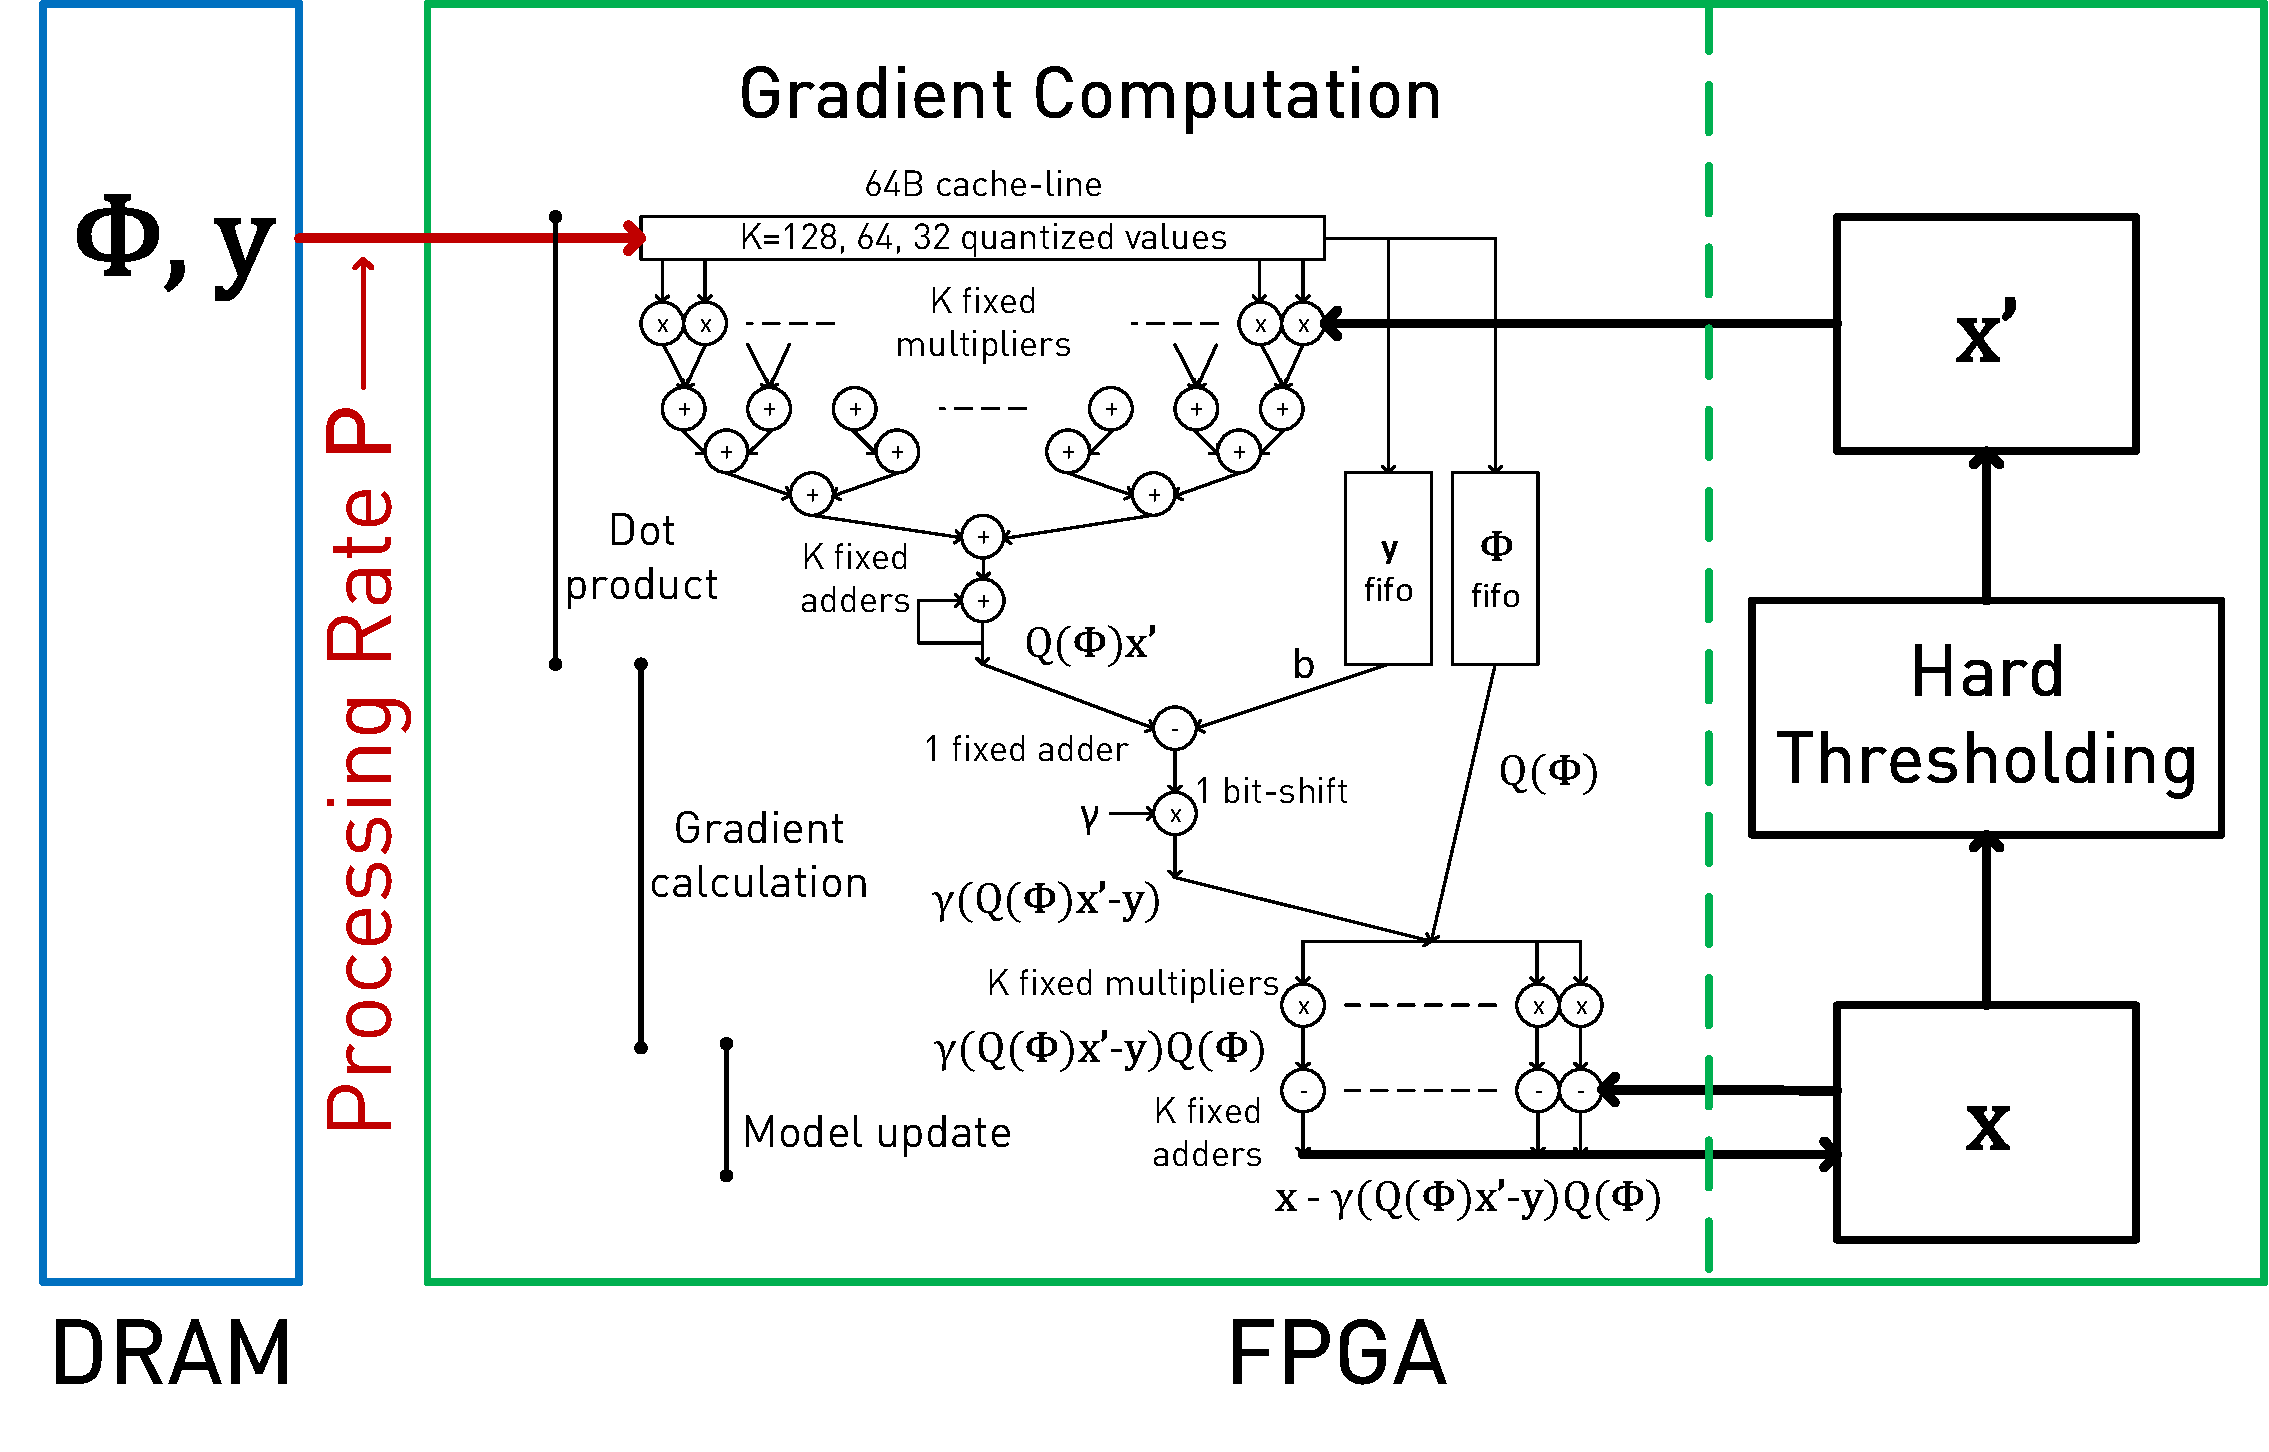
\includegraphics[width=0.9\columnwidth, angle=0]{figs/niht_fpga.eps}
\caption{IHT on an FPGA-based system.}
\label{fig:fpga}
\end{figure}


{\bf Performance analysis:} The gradient computation unit as shown in Figure~\ref{fig:fpga} reads the measurement matrix ${\bf \Phi}$ and the measurements ${\bf y}$ from main memory and keeps {\bf x} in on-chip memory. It is able to process data from memory at ${\bf P}=12.8\,GB/s$. Thus, the design is bound on ${\bf P}$ for processing ${\bf \Phi}$ and ${\bf y}$. We achieve speed-up by quantizing ${\bf \Phi}$, because the time for each epoch is given by
$T = size({\bf \Phi})/{\bf P}$, since $size({\bf y}) \ll size({\bf \Phi})$. The essential trick for achieving linear speed-up is keeping ${\bf P}$ constant as the precision of ${\bf \Phi}$ is lowered (${\bf P}\to \land \, size({\bf \Phi})\downarrow$), which leads to more values arriving within each line from main memory. ${\bf P}$ can be kept constant on an FPGA, because we can adapt the gradient computation unit's microarchitecture and increase its internal parallelism to handle more values per incoming line. This is like having the ability to change the width of a vectorized instruction, which on a fixed microarchitecture as in a CPU or GPU is not possible.


















\section{Experiments on a Real Telescope}\label{section_experiments}
We assess the empirical performance of our approach using the radio interferometer measurements from a real telescope: the LOw Frequency ARray (LOFAR). We first demonstrate that the accuracy achieved in the low precision setting is compatible with high precision IHT and the other state-of-art methods, and discuss the validity theoretical guarantees presented in Theorem~\ref{main_theorem_TH} for the telescope measurement matrix. Then we show the speed-up on FPGA.
\subsection{Accuracy of Sky Recovery}
We image the full sky by employing 30 low-band antennas of LOFAR CS302 station that operates in 15-80 MHz frequency band where the sky is populated with 30 strong sources where signal-to-noise ratio is 0 dB at the antenna level, i.e., $10\log_{10}(\|{\bf \Phi x}\|_2^2/\|{\bf e}\|_2^2) = 0$ dB. 
\subsubsection{Improving the least square estimates}
Fig.~\ref{fig:sky_images} provides an example of sky recoveries: (a) ground truth estimated over 12 hours of observation, (b) a least square estimate of underlying sky (or dirty image in the nomenclature of radio astronomy), (c) 32-bits, (d) 2-bits IHT and (e) the state-of-art interferometry imaging algorithm CLEAN. This experiment indicates that low precision IHT captures the sky sources successively even when only 2-bits are used to compress ${\bf \Phi}$. This suggest that we can drastically reduce the data precision yet still estimate the sky precisely.

\begin{figure*}\label{sky_images}
  \centering
    \includegraphics[width=1.02\textwidth]{figs/sky_images2.pdf}
  \caption{Sky recovery performances of high precision (32-bits), low precision (2-bits) IHT and CLEAN on a synthetic data setting populates with 30 celestial sources.}
  \label{fig:sky_images}
\end{figure*}

This empirical evidence is powerful yet not completely surprising. Mathematically, the measurement matrix we formed here hints on the distance between the antennas hence the phase relations. That is, each time a bit $r_{m, n}$ or $c_{m, n}$ flips its sign where $\hat{\bf \Phi}_{m, n} = r_{m, n} +j c_{m,n}$, $m = {1, 2, ..., M}$ and $n = {1, 2, ..., N}$, we approximately know the change in horizontal and vertical directions on the ground, preserving the phase information required for interferometric imaging even at very low precision.

Recall from the former discussions that noise in receivers is far stronger than the weak incoming signals thus low SNR at the antenna level results, i.e., usually ranged from -5 to 5 dB. Clearly, the CLEAN algorithm notably underperforms in the presence of significant noise. This undesirable property is yet not surprising. A careful look into the the algorithmic steps, it apparently matches also to the noise artefacts in the image considering them as a point source. This can also be justified mathematically: we designed the problem such that an execution of {CLEAN} corresponds to the first iteration recovery of IHT, which interprets our numerical results. 

%The reader might argue that, besides being on its most possible realistic setting, the above experiment does not fully capture the performance of low precision iht especially when only 2-bits are used to represent a dense measurement matrix. 

\subsubsection{Empirical comparison to other state-of-art methods}
This section dedicates in numerical comparisons of low precision to high precision IHT, CoSaMP and $\ell_1$-based approach. The thread that binds all of these approaches in this experiment is their capability of sparse signal recovery. For this particular formulation of the interferometric imaging problem, they can iteratively build up an estimate of sky map ${\bf x}$. In order to avoid creating bias towards any algorithm, we implement these algorithms in a fair setting.
\begin{figure}
\centering
\includegraphics[width=1.1\columnwidth, angle=0]{figs/comparison.pdf}
\caption{Recovery error and exact recovery performance. Comparison of 2-bits IHT to 32-bits IHT, CoSaMP, $\ell_1$-solution.}
\label{fig:comparison}
\end{figure}
We evaluate the algorithms through two different metrices: (1) the recovery error and (2) exact support recovery. In radio interferometry, however, it is customary to use number of true celestial sources resolved in the recovered image as a performance metric, i.e., true-positive findings. That is, the performance of the algorithms is no longer described by its ability to recover support entirely but the sky objects, which possess higher error tolerance. 

We demonstrate in Fig.~\ref{fig:comparison} that IHT performs as good as its alternatives and compatible to $\ell_1$-minimization in terms of its exact recovery performance. The empirical results suggest that the celestial sources can still be recovered by dramatically compressing ${\bf \Phi}$.

{\it Discussions on these results:} This experiment is informative merely on the accuracy of the results obtained implementing these alternative algorithms. A fair comparison involves the analysis of different properties such as speed and storage requirements, flexibility and ease of implementation. Capsulizing briefly, CoSaMP has strong theoretical guarantee when the least squares solution is supplied and requires the solution to an inverse problem at each iteration, which is costly in general and demands better storage capability~\cite{needel2008cosamp}. On the other hand, IHT is shown to outperform CoSaMP and have significant speed advantage~\cite{blumensath2012greedy} when ${\bf \Phi}$ has similar entries in magnitude, e.g., radio interferometer case. The empirical evidence further suggest that IHT performs nearly as well as the $\ell_1$-based approach. Referring back to Fig.~\ref{fig:sky_images}, the CLEAN requires a 2D Fourier inversion and deconvolution per iteration thus the operational expense of the method is relatively higher compared to those of IHT and CoSaMP~\cite{simeoni2015rai}. Sharing similar performance guarantees with the high precision IHT, low precision approach thus seems powerful considering all these aspects. This is evident in Fig.~\ref{fig:comparison}.


% \., which is vastly superior to the resitual in...
% This suggest we can drastically reduce bidi bidi
% Such a result has potentially profound consequences for the power consumption.


\subsubsection{Monitoring the Recovery Error}
Real-life problems usually lack of traditional RIP, that is, $\|{\bf \Phi}\|_2 < 1$. The scale-invariant feature of the measurement matrix used in normalized IHT however alleviates the RIP condition and imposes a fairly mild constraint in~\ref{rip_lowprecision}, i.e., non-symmetric RIP. In a series of paper~\cite{blumensath2010niht, blumensath2012greedy}, CoSaMP is shown to perform markedly worse when the RIP condition fails. IHT, however, still preserves its near-optimal recoveries far beyond the region of RIP. While this favors IHT over CoSaMP when applying to real-life problems, there is no rigid assumption imposed on $\ell_1$-minimization. Still \ref{rip} trivially holds.
% \begin{figure}[h!]
% \centering
% \includegraphics[width=1\columnwidth, angle=0]{figs/beta.pdf}
% \caption{Monitoring the error coefficients: $1/\beta_{2s}$ and $L/\hat{\beta}_{2s}$ that scale $ {\epsilon}_s$ and $ {\epsilon}_q$, respectively. Sparsity ratio stands for $2s/M$. The numerical value of coefficients guarantees that quantization error $ {\epsilon}_q$ is sufficiently small regardless of the number of bits used to represent ${\bf \Phi}$.}
% \label{fig:beta}
% \end{figure}
 Recall from Theorem~\ref{main_theorem_TH} that two conditions ensuring the performance guarantees are in order (a) $\gamma_{2s}, \hat{\gamma}_{2s} \leq 1/16$, (b) ${L}/{\hat{\beta}_{2s}2^{b_{\bf \Phi}}}$ must be sufficiently large to minimize quantization error $ {\epsilon}_q$. Fortunately, the image grid we initially form as well as scale-invariant property of normalized IHT yield us the control of $\gamma_{2s}, \hat{\gamma}_{2s}$ and $\hat{\beta}_{2s}$, respectively, through a pre-processing of ${\bf \Phi}$. Analytic derivations of these parameters is possible but intractable due to amount of nonlinear operations contained in the formulation of ${\bf \Phi}$. 
\begin{figure}[h!]
\centering
\includegraphics[width=1\columnwidth, angle=0]{figs/beta.pdf}
\caption{Monitoring the error coefficients: $1/\beta_{2s}$ and $L/\hat{\beta}_{2s}$ that scale $ {\epsilon}_s$ and $ {\epsilon}_q$, respectively. Sparsity ratio stands for $2s/M$. The numerical value of coefficients guarantees that quantization error $ {\epsilon}_q$ is sufficiently small regardless of the number of bits used to represent ${\bf \Phi}$.}
\label{fig:beta}
\end{figure}

In Fig.~\ref{fig:beta}, we numerically provide the scaling factors of errors $ {\epsilon}_s$ and $ {\epsilon}_q$: $1/\beta_{2s}$ and ${L}/{\hat{\beta}_{2s}}$, respectively. Theorem~\ref{main_theorem_TH} states that the recovery error is induced by the terms: $\|{\bf e} \|_2/|\beta_{2s}$ and $L\|{\bf x}^s \|_2/{\hat{\beta}_{2s}2^{b_{\bf \Phi}}}$. Therefore we investigate these scaling over various antenna numbers and sparsity level. The results suggest that 2-bits IHT has a negligible quantization error when applied radio interferometry imaging problem. We will now show the runtime improvement on FPGA.
\subsection{Speed-up on FPGA}
We demonstrate the speed up for performing IHT on the FPGA-based system in Fig.~\ref{fig:fpga_time}. We observe that quantization, and the resulting compression of the measurement matrix ${\bf \Phi}$ leads to linear speed up for recovering the support vector. As previously studied in the performance analysis part in Section~\ref{sec:fpga}, all variants (full precision to lowest precision) of IHT on FPGA can consume ${\bf \Phi}$ at the same rate, and therefore the runtime of IHT is linearly dependent on the size of ${\bf \Phi}$, thereby leading to linear speed ups that we observe in the experiments.

A subtle observation related to the particular system's characteristics: When comparing the runtime between 32-bit floating-point precision and 2-bit double sampled precision, we observe 7.7x speed up, although the data compression rate is 8x. The reason for that is, when using quantized ${\bf \Phi}$, the FPGA reads for each epoch a freshly quantized ${\bf \Phi}$ (due to stochastic quantization) and therefore reads from a different location in main memory; whereas when using full-precision ${\bf \Phi}$, the FPGA always reads from the same location in main memory, utilizing the cache more efficiently. This is the reason, why the speed up rate is not perfectly matching the compression rate.


\begin{figure}[h!]
\centering
\includegraphics[width=1.1\columnwidth, angle=0]{figs/fpga_final.pdf}
\caption{Speed-up achievements of low precision IHT on FPGA. 2-bits IHT provides 7.7x runtime efficiency.}
\label{fig:fpga_time}
\end{figure}
\section{Discussion}\label{section_discussion}
Motivated by the question "How can we efficiently transmit and process enormous amount of telescope data?", we investigate the applicability of low precision scheme to the applications that are essentially sparse signal recovery problems. Our algorithm performed far beyond what we anticipated.

IHT for compressive sensing was rigorously shown to retain uniform convergence guarantees at low precision. An application to radio astronomy validated our claim and showed that the heuristic and rigorous arguments are in agreement with experiments. The results bear out that our approach offers similar accuracy with the high precision IHT even with far less precision of data points. A fundamental contribution was to show that even using 2-bits to represent data hence significant speed-up on hardware, accuracy of sparse approximations can still be preserved.

Our next question is: Can end-to-end low precision data representation enable the same?
\bibliography{references}
\bibliographystyle{icml2018}
\end{document} 

